\documentclass{beamer}
\usetheme{metropolis}
\setbeamertemplate{navigation symbols}{}

\usepackage[utf8]{inputenc}
\usepackage[T1]{fontenc}
\usepackage[polish]{babel}
\usepackage{hyperref}
\usepackage{xcolor}
\usepackage{graphicx}

% Metropolis theme options
\metroset{block=fill}
\metroset{progressbar=frametitle}

\title{Co robić na studiach, żeby było co wpisać do CV}
\author{Vlad Snozyk}
\date{Kacwin, 2025}

\begin{document}

\begin{frame}
  \titlepage
\end{frame}

% Slide 2
\begin{frame}{Motywacja}
  \centering
  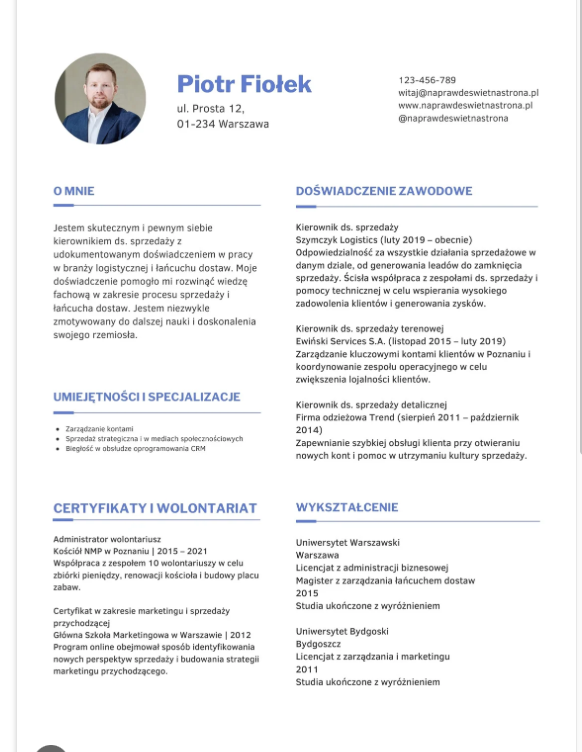
\includegraphics[width=0.8\textwidth]{cv1.png}
\end{frame}

% Slide 3
\begin{frame}{Motywacja}
  \centering
  
\includegraphics[width=0.8\textwidth]{cv2.png}
\end{frame}

% Slide 4
\begin{frame}{Dla kogo prezentacja?}
  \centering
\end{frame}

% Slide 5
\begin{frame}{Członkowstwo w kołach naukowych}
  \centering
  
\includegraphics[width=0.8\textwidth]{knmf.jpg}
\end{frame}

% Slide 6
\begin{frame}{Dobieranie dodatkowych przedmiotów na uczelni}
  \begin{enumerate}
    \item Programowanie w języku Python
    \item Programowanie w języku R
    \item Sieci neuronowe
    \item Sterowanie stochastyczne w czasie ciągłym
    \item Inżynieria finansowa
    \item Arbitrage theory
  \end{enumerate}
\end{frame}

% Slide 7
\begin{frame}{Projekty na GitHubie (Przedmioty z projektami)}
  \centering
  
\includegraphics[width=0.5\textwidth]{github_logo.png}
\end{frame}

% Slide 8
\begin{frame}{Platforma Project Euler}
  \centering
  
\includegraphics[width=0.6\textwidth]{euler.png}
\end{frame}

% Slide 9
\begin{frame}{Konkursy (Prosperity)}
  \centering
  
\includegraphics[width=0.8\textwidth]{prosperity.png}
\end{frame}

% Slide 10
\begin{frame}{Kaggle}
  \centering
  
\includegraphics[width=0.5\textwidth]{kaggle_logo.png}
\end{frame}

% Slide 11
\begin{frame}{numer.ai}
  \centering
  
\includegraphics[width=0.5\textwidth]{numerai_logo.png}
\end{frame}

% Slide 12
\begin{frame}{Slajd o miłości}
  \centering
  
\includegraphics[width=0.5\textwidth]{heart.png}
\end{frame}

% Slide 13
\begin{frame}{Pytania}
  \centering
  \Large
  Czy są jakieś pytania?
\end{frame}

% Slide 14
\begin{frame}{Podziękowanie}
  \centering
  \Large
  Dziękuję.
\end{frame}

\end{document}
